%
% einleitung.tex -- Beispiel-File für die Einleitung
%
% (c) 2020 Prof Dr Andreas Müller, Hochschule Rapperswil
%
% !TEX root = ../../buch.tex
% !TEX encoding = UTF-8
%
\subsection{Kugel\label{geodaeten:section:Standardverfahren:Kugel}}
\rhead{Standardverfahren Beispiele}

Intuitiv erwarten wir, dass die Geodäten auf der Kugeloberfläche Grosskreise sind.
Ein Grosskreis ist der geradlinigste Weg zwischen zwei Punkten auf einer Kugel.
Dies kann man sich vorstellen, indem man zwei Nadeln in eine Kugeloberfläche steckt und einen Faden um die beiden Nadeln spannt.
Der Faden wird immer entlang eines Grosskreises verlaufen.
Tatsächlich folgen Flugzeuge auf Langstreckenflügen dieser Logik und fliegen entlang von Grosskreisen, um die kürzeste Strecke zwischen zwei Punkten auf der Erde zurückzulegen.
Wir möchten nun überprüfen, ob wir mit dem Standardverfahren tatsächlich zu dieser Lösung kommen.

Um dies zu tun, benötigen wir den bereits im vorherigen Abschnitt hergeleiteten metrischen Tensor für die Kugeloberfläche.
Dieser ist in Kugelkoordinaten $(\theta, \phi)$ gegeben durch
\begin{equation}
	g_{ij} = r^2 \begin{pmatrix}
		1 & 0 \\
		0 & \sin^2\theta
	\end{pmatrix}.
\end{equation}

Zuerst berechnen wir die Inverse des metrischen Tensors, da diese für die Berechnung der Christoffel-Symbol benötigt wird.
Der inverse Tensor $g^{ij}$ ist ergibt sich zu
\begin{equation}
	g^{ij} = \frac{1}{r^2} 
	\begin{pmatrix}
		1 & 0 \\
		0 & \frac{1}{\sin^2\theta}
	\end{pmatrix}.
	\label{geodaeten:equation:StaKugel:TensorInverse}
\end{equation}

Nun berechnen wir die partiellen Ableitungen des metrischen Tensors $g_{ij}$ in Bezug auf die Koordinaten $\theta$ und $\phi$.
Da $g_{11} = r^2$ und $g_{22} = r^2 \sin^2\theta$, erhalten wir
\begin{equation}
	\frac{\partial g_{11}}{\partial \theta} = 0, \quad \frac{\partial g_{11}}{\partial \phi} = 0, \quad \frac{\partial g_{22}}{\partial \theta} = 2r^2 \sin\theta \cos\theta, \quad \frac{\partial g_{22}}{\partial \phi} = 0.
	\label{geodaeten:equation:StaKugel:Ableitungen}
\end{equation}

\subsection{Christoffel-Symbole}
Mit den Ableitungen \eqref{geodaeten:equation:StaKugel:Ableitungen} und dem inversen Tensor $g^{ij}$ \eqref{geodaeten:equation:StaKugel:TensorInverse} können wir nun die Christoffel-Symbole berechnen durch
\begin{equation}
	\Gamma_{ij}^k = \frac{1}{2} g^{kl} \left( \frac{\partial g_{jl}}{\partial u^i} + \frac{\partial g_{il}}{\partial u^j} - \frac{\partial g_{ij}}{\partial u^l} \right),
\end{equation}
wobei $u^1 = \theta$ und $u^2 = \phi$.

Nach Einsetzen der Werte und Vereinfachung erhalten wir folgende nicht-verschwindende Christoffel-Symbole
\begin{equation}
	\Gamma_{12}^2 = \Gamma_{21}^2 = \cot\theta \quad \text{und} \quad \Gamma_{22}^1 = -\sin\theta \cos\theta.
\end{equation}

Anders als im Fall des Zylinders, wo der metrische Tensor konstant war, führt die Abhängigkeit des metrischen Tensors von der Koordinate $\theta$ zu nicht-verschwindenden Christoffel-Symbolen, welche die intrinsische Krümmung der Kugeloberfläche beschreiben.

Um diese Krümmung zu verstehen, betrachten wir die Bewegung eines Tangentialvektors auf der Oberfläche in Bezug auf die Basisvektoren.

Wird die Komponente des Vektors entlang eines Breitenkreises verändert, also in $\phi$-Richtung, führt das zu keiner Änderung der Vektorrichtung, da das Bogenmass von $\phi$ entlang eines Breitenkreises konstant bleibt.
Diese Bewegung beeinflusst die allgemeine Richtung des Vektors also nicht, was auch im metrischen Tensor reflektiert wird, der keinerlei Abhängigkeit von $\phi$ aufweist.

Andererseits führt eine Veränderung der Komponente entlang eines Längengrades, also in $\theta$-Richtung, zu einer Veränderung der Vektorrichtung.
Dies liegt daran, dass das Bogenmass von $\phi$ mit $\theta$ variiert: 
Je näher man den Polen kommt, desto kürzer wird der Bogen für eine gegebene Änderung von $\theta$, was die Gesamtrichtung des Vektors beeinflusst. 
Damit der Tangentialvektor seine ursprüngliche Richtung beibehält, müsste die Bewegung in der $\phi$-Richtung zunehmend verringert werden, je näher man den Polen kommt.

Diese Richtungsänderung des Vektors ist eine direkte Folge der intrinsischen Krümmung der Kugeloberfläche.
Die nicht-verschwindenden Christoffel-Symbole beschreiben genau diese Krümmung und geben an, wie sich die Richtung eines Vektors bei seiner Bewegung entlang der Oberfläche verändert.

\subsection{Geodätengleichung}
Mit den berechneten Christoffel-Symbolen können wir nun die Geodätengleichungen für die Kugeloberfläche aufstellen.

Die allgemeine Form der Geodätengleichung lautet
\begin{equation}
	\ddot{u}^k + \Gamma^k_{ij} \dot{u}^i \dot{u}^j = 0,
\end{equation}
wobei $u^k$ die Koordinaten darstellen, in diesem Fall $\theta$ und $\phi$.

Setzen wir die entsprechenden Christoffel-Symbole und Koordinaten in die Gleichungen ein, erhalten wir
\begin{equation}
	\begin{aligned} 
		0 &= \ddot{\theta} + \Gamma^1_{11} \dot{\theta} \dot{\theta} + 2\Gamma^1_{12} \dot{\theta}\dot{\phi} + \Gamma^1_{22} \dot{\phi} \dot{\phi} \\
		0 &= \ddot{\phi} + \Gamma^2_{11} \dot{\theta} \dot{\theta} + 2\Gamma^2_{12} \dot{\theta}\dot{\phi} + \Gamma^2_{22} \dot{\phi} \dot{\phi},
	\end{aligned}
\end{equation}
und weil einige der Christoffel-Symbole Null sind, vereinfachen sich die Geodätengleichungen schliesslich zu
\begin{align}
	0 &= \ddot{\theta} - \sin\theta \cos\theta \, \dot{\phi}^2 \\
	0 &= \ddot{\phi} + 2 \cot\theta \, \dot{\theta} \dot{\phi}.
\end{align}

Da $r$ lediglich ein Skalierungsfaktor ist, kürzt es sich in den Geodätengleichungen heraus. 
Die Geometrie wird allein durch die Winkelabhängigkeit bestimmt, sodass der Radius keinen Einfluss auf die Form der Geodäten hat.

Das Lösen der Geodätengleichungen ist oft aufwendig und schwierig, was numerische Ansätze erforderlich macht. 
Daher überprüfen wir durch Analyse, ob Grosskreise diese tatsächlich erfüllen und als Lösungen gelten.

\subsection{Äquator}
Betrachten wir die Geodätengleichungen für konstantes $\theta$, also entlang eines Breitengrads.
Für konstantes $\theta$ gilt $\dot{\theta} = 0$ und $\ddot{\theta} = 0$.
Setzen wir dies in die erste Geodätengleichung ein, so erhalten wir:
\begin{equation}
	0 = -\sin\theta \cos\theta \, \dot{\phi}^2.
\end{equation}
Die zweite Geodätengleichung vereinfacht sich zu $0 = \ddot{\phi}$, was zeigt, dass $\phi(t)$ linear in der Zeit variiert.
Diese erste Geodätengleichung wird nur für $\theta = \frac{\pi}{2}$ erfüllt, das heisst, nur für den Äquator.
Für alle anderen Breitengrade mit $\theta \neq \frac{\pi}{2}$ muss $\dot{\phi}$ gleich null werden, was bedeutet, dass es keine Bewegung in der $\phi$-Richtung gibt und somit keine Geodäte vorliegt.
Der Äquator, als einziger Breitengrad, erfüllt daher die Geodätengleichungen und ist ein Grosskreis.

\begin{figure}
	\centering
	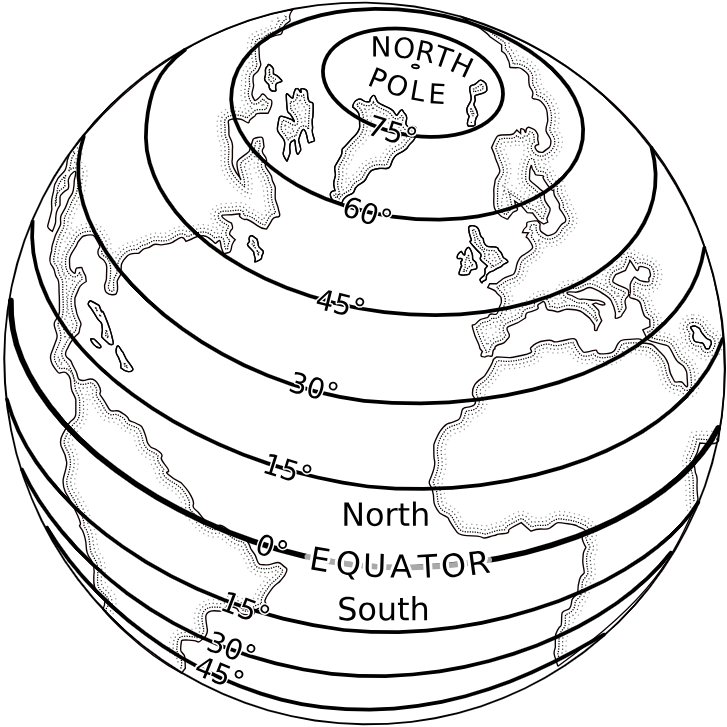
\includegraphics[width=7cm]{papers/geodaeten/Abbildungen/Standardverfahren/StaKugelBreitengrade}
	\caption{Erdkugel mit Breitengrade und Äquator als Geodätenlinie}
	\label{geodaeten:figure:Standardverfahren:Breitengrade}
\end{figure}

\subsection{Längengrade}
Nun analysieren wir die Geodätengleichungen für konstantes $\phi$, also entlang eines Längengrads.
Für konstantes $\phi$ gilt $\dot{\phi} = 0$ und $\ddot{\phi} = 0$.
Setzen wir dies in die erste Geodätengleichung ein, erhalten wir:
\begin{equation}
	\ddot{\theta} = 0,
\end{equation}
was bedeutet, dass $\theta(t)$ linear in der Zeit variiert.
Die zweite Geodätengleichung wird ebenfalls trivial erfüllt, da $\dot{\phi} = 0$ und somit keine Beschleunigung in der $\phi$-Richtung vorliegt.
Damit sind alle Längengrade tatsächlich Geodäten.

Zusammenfassend konnten wir durch unsere Analyse zeigen, dass nur Grosskreise, wie der Äquator und die Längengrade, die Geodätengleichungen vollständig erfüllen und somit die wahren Geodäten auf der Kugeloberfläche darstellen.

Wir haben damit erfolgreich nachgewiesen, dass die Lösungen der Geodätengleichungen $\theta(t)$ und $\phi(t)$ zwangsläufig die Form von Grosskreisen annehmen müssen und dass die allgemeine Geodätengleichung diese Grosskreise korrekt als die Geodäten auf der Kugeloberfläche identifiziert.

\begin{figure}
	\centering
	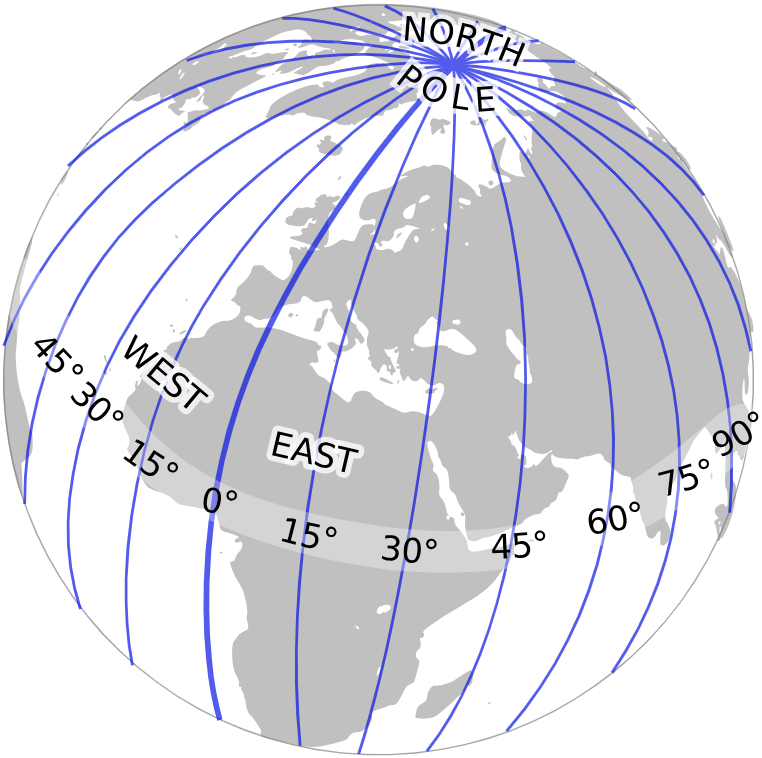
\includegraphics[width=7cm]{papers/geodaeten/Abbildungen/Standardverfahren/StaKugelLaengengrade}
	\caption{Erdkugel mit Längengrade als Geodätenlinen}
	\label{geodaeten:figure:Standardverfahren:Laengengrade}
\end{figure}